\documentclass[journal,12pt,twocolumn]{IEEEtran}
\usepackage{cite}
\usepackage{amsmath,amssymb,amsfonts,amsthm}
\usepackage{algorithmic}
\usepackage{graphicx}
\usepackage{textcomp}
\usepackage{xcolor}
\usepackage{txfonts}
\usepackage{listings}
\usepackage{enumitem}
\usepackage{mathtools}
\usepackage{gensymb}
\usepackage[breaklinks=true]{hyperref}
\usepackage{tkz-euclide} % loads  TikZ and tkz-base
\usepackage{listings}
\usepackage{floatrow}  


\newtheorem{theorem}{Theorem}[section]
\newtheorem{problem}{Problem}
\newtheorem{proposition}{Proposition}[section]
\newtheorem{lemma}{Lemma}[section]
\newtheorem{corollary}[theorem]{Corollary}
\newtheorem{example}{Example}[section]
\newtheorem{definition}[problem]{Definition}
%\newtheorem{thm}{Theorem}[section] 
%\newtheorem{defn}[thm]{Definition}
%\newtheorem{algorithm}{Algorithm}[section]
%\newtheorem{cor}{Corollary}
\newcommand{\BEQA}{\begin{eqnarray}}
\newcommand{\EEQA}{\end{eqnarray}}
\newcommand{\define}{\stackrel{\triangle}{=}}
\theoremstyle{remark}
\newtheorem{rem}{Remark}

%\bibliographystyle{ieeetr}
\begin{document}
%


\providecommand{\pr}[1]{\ensuremath{\Pr\left(#1\right)}}
\providecommand{\prt}[2]{\ensuremath{p_{#1}^{\left(#2\right)} }}        % own macro for this question
\providecommand{\qfunc}[1]{\ensuremath{Q\left(#1\right)}}
\providecommand{\sbrak}[1]{\ensuremath{{}\left[#1\right]}}
\providecommand{\lsbrak}[1]{\ensuremath{{}\left[#1\right.}}
\providecommand{\rsbrak}[1]{\ensuremath{{}\left.#1\right]}}
\providecommand{\brak}[1]{\ensuremath{\left(#1\right)}}
\providecommand{\lbrak}[1]{\ensuremath{\left(#1\right.}}
\providecommand{\rbrak}[1]{\ensuremath{\left.#1\right)}}
\providecommand{\cbrak}[1]{\ensuremath{\left\{#1\right\}}}
\providecommand{\lcbrak}[1]{\ensuremath{\left\{#1\right.}}
\providecommand{\rcbrak}[1]{\ensuremath{\left.#1\right\}}}
\newcommand{\sgn}{\mathop{\mathrm{sgn}}}
\providecommand{\abs}[1]{\left\vert#1\right\vert}
\providecommand{\res}[1]{\Res\displaylimits_{#1}} 
\providecommand{\norm}[1]{\left\lVert#1\right\rVert}
%\providecommand{\norm}[1]{\lVert#1\rVert}
\providecommand{\mtx}[1]{\mathbf{#1}}
\providecommand{\mean}[1]{E\left[ #1 \right]}
\providecommand{\cond}[2]{#1\middle|#2}
\providecommand{\fourier}{\overset{\mathcal{F}}{ \rightleftharpoons}}
\newenvironment{amatrix}[1]{%
  \left(\begin{array}{@{}*{#1}{c}|c@{}}
}{%
  \end{array}\right)
}
%\providecommand{\hilbert}{\overset{\mathcal{H}}{ \rightleftharpoons}}
%\providecommand{\system}{\overset{\mathcal{H}}{ \longleftrightarrow}}
	%\newcommand{\solution}[2]{\textbf{Solution:}{#1}}
\newcommand{\solution}{\noindent \textbf{Solution: }}
\newcommand{\cosec}{\,\text{cosec}\,}
\providecommand{\dec}[2]{\ensuremath{\overset{#1}{\underset{#2}{\gtrless}}}}
\newcommand{\myvec}[1]{\ensuremath{\begin{pmatrix}#1\end{pmatrix}}}
\newcommand{\mydet}[1]{\ensuremath{\begin{vmatrix}#1\end{vmatrix}}}
\newcommand{\myaugvec}[2]{\ensuremath{\begin{amatrix}{#1}#2\end{amatrix}}}
\providecommand{\rank}{\text{rank}}
\providecommand{\pr}[1]{\ensuremath{\Pr\left(#1\right)}}
\providecommand{\qfunc}[1]{\ensuremath{Q\left(#1\right)}}
	\newcommand*{\permcomb}[4][0mu]{{{}^{#3}\mkern#1#2_{#4}}}
\newcommand*{\perm}[1][-3mu]{\permcomb[#1]{P}}
\newcommand*{\comb}[1][-1mu]{\permcomb[#1]{C}}
\providecommand{\qfunc}[1]{\ensuremath{Q\left(#1\right)}}
\providecommand{\gauss}[2]{\mathcal{N}\ensuremath{\left(#1,#2\right)}}
\providecommand{\diff}[2]{\ensuremath{\frac{d{#1}}{d{#2}}}}
\providecommand{\myceil}[1]{\left \lceil #1 \right \rceil }
\newcommand\figref{Fig.~\ref}
\newcommand\tabref{Table~\ref}
\newcommand{\sinc}{\,\text{sinc}\,}
\newcommand{\rect}{\,\text{rect}\,}
%%
%	%\newcommand{\solution}[2]{\textbf{Solution:}{#1}}
%\newcommand{\solution}{\noindent \textbf{Solution: }}
%\newcommand{\cosec}{\,\text{cosec}\,}
%\numberwithin{equation}{section}
%\numberwithin{equation}{subsection}
%\numberwithin{problem}{section}
%\numberwithin{definition}{section}
%\makeatletter
%\@addtoreset{figure}{problem}
%\makeatother

%\let\StandardTheFigure\thefigure
\let\vec\mathbf


\bibliographystyle{IEEEtran}


\vspace{3cm}

\title{
%	\logo{
Assignment 1
%	}
}
\author{ EE22BTECH11053 - Tanmay Vishwasrao% <-this % stops a space
	
}	

\maketitle

\newpage

%\tableofcontents

\bigskip

\renewcommand{\thefigure}{\theenumi}
\renewcommand{\thetable}{\theenumi}
Question 1.5.9\\
Find the other points of contact $\vec{E}_3$ and $\vec{F}_3$.

\solution
From the previous references we have the value of Incentre $\vec{I}$ is
\begin{align}
\vec{I} &=\myvec{-1.4775\\-0.7949}
\end{align}
And the value of inradius $r$ is 1.8969. The parametric equation of line is:
\begin{align}
&= \vec{A}+k\vec{m}
\end{align}
The equation of Incircle is given by:
\begin{align}
\norm{\vec{x}-\vec{I}}^2 &= r^2
\end{align}
Since its a parametric equation we can substitute $(3)$ as $\vec{x}$ in $(4)$.
\begin{align}
\norm{\vec{A}+k\vec{m}-\vec{I}}^2 &= r^2 \\
\brak{\vec{A}+k\vec{m}-\vec{I}}^\top\brak{\vec{A}+k\vec{m}-\vec{I}} &= r^2
\end{align}
On simplifying the above equation:
\begin{align}
k^2\norm{\vec{m}}^2+2k\brak{\vec{m}}^\top\brak{\vec{A-I}}+\norm{\vec{I}}^2 \nonumber \\
+\norm{\vec{A}}^2-2\brak{\vec{A}^\top\vec{I}}-r^2 &= 0
\label{eq:equation}
\end{align}
\begin{enumerate}
\item Finding the point $\vec{E}_3$.\\
The equation of $\vec{E}_3$:
\begin{align}
\vec{E}_3 &=\vec{A}+k\vec{m}
\end{align}
Where 
\begin{align}
\vec{m} = \vec{A}-\vec{B}
\end{align}
Now putting the values of $\vec{A}, \vec{m}, \vec{I}$ in \eqref{eq:equation}.
\begin{align}
74k^2+27.6463k+2.5821 &= 0
\end{align}
Discriminant of the above equation is:
\begin{align}
D &= \brak{27.6463}^2-4\brak{74}\brak{2.5821}\\
&= 764.3179-764.3179\\
&= 0
\end{align}
Since the discriminant is $0$. The value of k will be:
\begin{align}
k &= -\frac{2\brak{\vec{m}}^\top\brak{\vec{A-I}}}{2\norm{\vec{m}}^2} \\
&= -\frac{27.6463}{148} \\
&= -0.1867
\end{align}
Now we can find $\vec{E}_3$ using above results:
\begin{align}
\vec{E}_3 &=\myvec{1\\-1}-0.1867\myvec{5\\-7} \\
&=\myvec{0.066\\0.307}
\end{align}
\item Finding the point $\vec{F}_3$.\\
For the point $\vec{F}_3$ the value of $\vec{m} = \vec{A}-\vec{C}$. 
\begin{align}
\vec{F}_3 &=\vec{A}+k\vec{m}
\end{align}
Now putting the values of $\vec{A}, \vec{m}, \vec{I}$ in \eqref{eq:equation}.
\begin{align}
32k^2+18.1801k+2.5821 &= 0
\end{align}
Discriminant of the above equation is:
\begin{align}
D &= \brak{18.1801}^2-4\brak{32}\brak{2.5821}\\
&= 330.51-330.51\\
&= 0
\end{align}
Since the discriminant is $0$. The value of k will be:
\begin{align}
k &= -\frac{2\brak{\vec{m}}^\top\brak{\vec{A-I}}}{2\norm{\vec{m}}^2}\\
&= -\frac{18.1801}{64}\\
&= -0.2840
\end{align}
Now we can find $\vec{F}_3$ using above results:
\begin{align}
\vec{F}_3 &=\myvec{1\\-1}-0.2840\myvec{4\\4}\\
&= \myvec{-0.136\\-2.136}
\end{align}
\end{enumerate}
\begin{figure}[H]
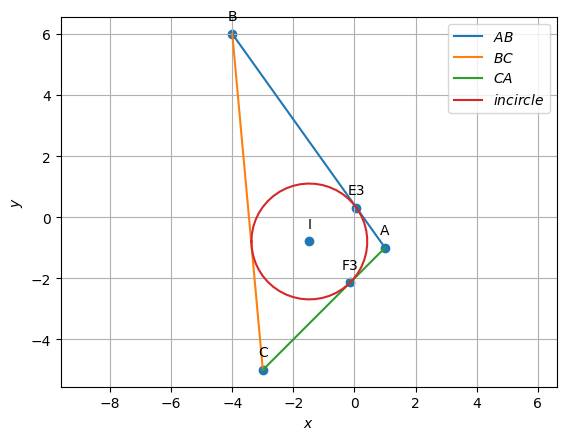
\includegraphics[width=\columnwidth]{figs/Incircle.png}
\caption{Points $\vec{E}_3$ and $\vec{F}_3$ plotted using python}
\label{fig:i_tri_py}
\end{figure}
\end{document}